\documentclass[12pt]{article}
\usepackage[utf8]{inputenc}
\usepackage{float}
\usepackage{amsmath}
\usepackage{enumerate}
\usepackage{tikz}
\usepackage{tikz-qtree}
\usetikzlibrary{automata,positioning}
\usepackage{tabularx}

\usepackage[hmargin=3cm,vmargin=6.0cm]{geometry}
%\topmargin=0cm
\topmargin=-2cm
\addtolength{\textheight}{6.5cm}
\addtolength{\textwidth}{2.0cm}
%\setlength{\leftmargin}{-5cm}
\setlength{\oddsidemargin}{0.0cm}
\setlength{\evensidemargin}{0.0cm}

%misc libraries goes here
\usepackage{tikz}
\usetikzlibrary{automata,positioning}

\begin{document}

\section*{Student Information} 
%Write your full name and id number between the colon and newline
%Put one empty space character after colon and before newline
Full Name : Yaşar Cahit Yıldırım \\
Id Number : 2310647
% Write your answers below the section tags
\section*{Answer 1}

\subsection*{a.}
	\begin{enumerate}[(i)]
		\item
		Let
		\begin{minipage}{0.4\textwidth}
			\vspace*{0.5cm}
			$$S_1 \rightarrow aS_1a\ |\ bS_2$$
			$$S_2 \rightarrow aS_2a\ |\ b$$
		\end{minipage}
		in 
		\begin{minipage}{0.5\textwidth}
			$\ G = \Big(V=\{S_1, S_2, a, b\}, \Sigma=\{a, b\}, R, S_1\Big)$
		\end{minipage}
		
		\item
		Let
		\begin{minipage}{0.4\textwidth}
			\vspace*{1.25cm}
			$$S_1 \rightarrow aS_2aS_2a\ |\ bS_2bS_2b$$
			$$S_2 \rightarrow aS_2a\ |\ aS_2b\ |\ bS_2a\ |\ bS_2b\ |\ a$$
			$$S_3 \rightarrow aS_3a\ |\ aS_3b\ |\ bS_3a\ |\ bS_3b\ |\ b$$
		\end{minipage}
		in 
		\begin{minipage}{0.5\textwidth}
			$\ G = \Big(V=\{S_1, S_2, S_3, a, b\}, \Sigma=\{a, b\}, R, S_1\Big)$
		\end{minipage}

		\vspace*{-1.5cm}
		
		\item
		Let
		\begin{minipage}{0.4\textwidth}
			\vspace*{2.7cm}
			$$S_1 \rightarrow S_2C\ |\ S_3C\ |\ AS_4\ |\ AS_5$$
			$$S_2 \rightarrow a\ |\ aS_2\ |\ aS_2b$$
			$$S_3 \rightarrow b\ |\ S_3b\ |\ aS_3b$$
			$$S_4 \rightarrow b\ |\ bS_4\ |\ bS_4c$$
			$$S_5 \rightarrow c\ |\ S_5c\ |\ bS_5c$$
		\end{minipage}
		\hspace{-0.75cm}
		in 
		\begin{minipage}{0.6\textwidth}
			$\ G = \Big(V=\{S_1, S_2, S_3, S_4, s_5, a, b, c\}, \Sigma=\{a, b, c\}, R, S_1\Big)$
		\end{minipage}

		\vspace*{-1cm}

		\item
		Let
		\begin{minipage}{0.4\textwidth}
			\vspace*{2.1cm}
			$$S_1 \rightarrow S_2S_3$$
			$$S_2 \rightarrow S_2S_4\ |\ \epsilon$$
			$$S_3 \rightarrow aS_3a\ |\ bS_3b\ |\ acS_2ca\ |\ bcS_2cb$$
			$$S_4 \rightarrow aS_4\ |\ bS_4\ |\ ac\ |\ bc$$
		\end{minipage}
		\hspace{-0.5cm}
		in 
		\begin{minipage}{0.6\textwidth}
			$\ G = \Big(V=\{S_1, S_2, S_3, S_4, a, b, c\}, \Sigma=\{a, b, c\}, R, S_1\Big)$
		\end{minipage}
	\end{enumerate}
	%\newpage

\subsection*{b.}
	\qquad We are dealing with sets so we can prove this by set equality. Let our language be $L$.\\

	\subsection*{ $\mathcal{L}(G) \subseteq L$: }

		\qquad Let's examine our grammar a bit. If we ignore the transitions $A \rightarrow BAA$ and $B \rightarrow ABB$ we can easily see that $A$ is a state which we come with one less $a$ than there are $b$'s from state S. And in this state we either finish the string with an $a$ or add an $a$ and return to the start state. $B$ is the same as $A$ with $b$'s so these two are used to balance the number of $a$'s and $b$'s.\\

		\qquad Now if we consider the $A \rightarrow BAA$ case with the help of above understandment, one $B$ and two $A$'s will in the long run result us with two extra $a$'s and one extra $b$ \textbf{from the numbers we are on}. Meaning that whatever depth the recursion will be, at the end we will get our two $a$ and one $b$ terminals in order for recursion to end. The same will apply to $B \rightarrow ABB$. We can conclude that whatever string our grammar create, it will be in the language, thus $\mathcal{L}(G) \subseteq L$.

	\subsection*{ $L \subseteq \mathcal{L}(G)$: }

		\qquad We can use induction to show this is the case.
		\begin{center}
				\textbf{Base Case:} Smallest nonempty strings in our language are $ab$ and $ba$, these are in our grammar.\\
				\textbf{Inductive Hypothesis:} Let's assume all words $w$ where $|w| \leq n$ in the language can be created by our grammar.\\
				\textbf{Inductive Proof:} Let's consider a word $w$ with $|w| = n+2$, $w$ either starts with an $a$ or $b$. If it starts with an $a$ it can be split as $aubv$ where $u,v\in L$ and $S \Rightarrow aB \Rightarrow aABB \Rightarrow aABbS$. $v$ equals to $S$ and $|v| \leq n$ so it can be created. We know $A$ creates strings that has one more $a$ and $B$ strings that has one more $b$. So $u = AB$ where $|v| \leq n$ is created also. Same applies if $w$ starts with a $b$, we split it as $buav$ and $bBAaS$. Thus $L \subseteq \mathcal{L}(G)$.\\
				Since $\mathcal{L}(G) \subseteq L$ and $L \subseteq \mathcal{L}(G)$, $L = \mathcal{L}(G)$
			\end{center}

\vspace{1.5cm}
\section*{Answer 2}

\subsection*{a.}
	\qquad The string $aab$ is an example. It's two leftmost derivations are:\\
	
	\begin{minipage}{\textwidth}
		\vspace*{-0.75cm}
		\hspace*{0.5cm}
		\Tree [.S [.A [.A [.a ] ] [.a ] ] [.b ] ]
		\hspace*{1cm}
		\begin{minipage}{0.3\textwidth}
			\vspace*{2cm}
			$S \Rightarrow Ab \Rightarrow Aab \Rightarrow aab$
		\end{minipage}
		\hspace*{1cm}
		\Tree [.S [.a ] [.a ] [.B [.b ] ] ]
		\hspace*{1cm}
		\begin{minipage}{0.3\textwidth}
			\vspace*{2cm}
			$S \Rightarrow aab \Rightarrow aab$
		\end{minipage}
	\end{minipage}
\vspace{-0.5cm}
\subsection*{b.}
	\qquad The $B$ non-terminal is not necessary because it only leads to create the word $aab$ but $aab$ is already accepted by different derivations. So an equivalent unambiguous CFG is simply:
	$$ G' = \{V' = \{a, b, S, A\}, \Sigma, R' = \{S \rightarrow Ab, A \rightarrow a \ Aa\}, S\}$$
\subsection*{c.}
	\begin{minipage}{\textwidth}
		\vspace*{-0.75cm}
		\hspace*{0.5cm}
		\Tree [.S [.A [.A [.a ] ] [.a ] ] [.b ] ]
		\hspace*{1cm}
		\begin{minipage}{0.3\textwidth}
			\vspace*{2cm}
			$S \Rightarrow Ab \Rightarrow Aab \Rightarrow aab$
		\end{minipage}
	\end{minipage}

\section*{Answer 3}

\subsection*{a.}
	$$\{a^{2n}b^{3n}\ |\ n \geq 0\}$$

\subsection*{b.}
	\qquad In the PDA, * symbol is used as "any symbol from alphabet" and + symbol as "just an allocator". 
	$$\{w_1w_2 \in \{a,b\}^*\ \big|\ |w_1w_2|\ \text{is odd or}\ (|w_1| = |w_2|\ \text{and}\ w_1 \neq w_2)\}$$
	% Sample empty diagram for your convenience, edit/use as you wish.
	\tikzset{every loop/.style={min distance=10mm,looseness=10}}
	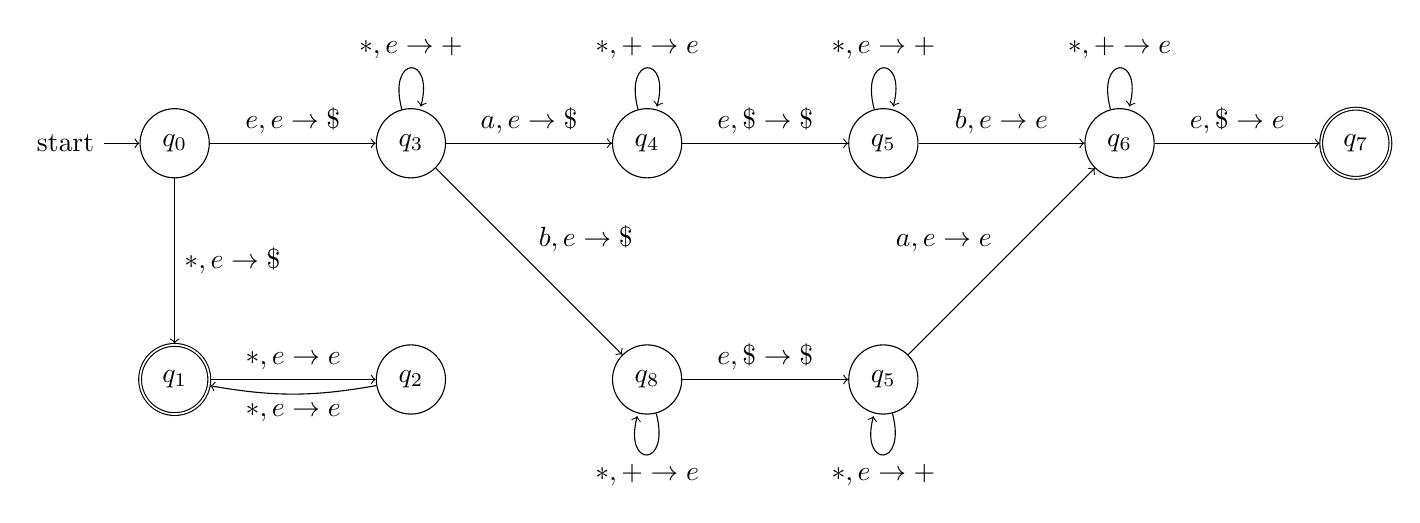
\begin{tikzpicture}[node distance=3cm,on grid,auto] 
		\node[state,initial   ]    (q0)                        {$q_0$};
		\node[state, accepting]    (q1) [below of=q0]          {$q_1$};
		\node[state           ]    (q2) [right of=q1]          {$q_2$};
		\node[state           ]    (q3) [right of=q0]          {$q_3$};
		\node[state           ]    (q4) [right of=q3]          {$q_4$};
		\node[state           ]    (q5) [right of=q4]          {$q_5$};
		\node[state           ]    (q6) [right of=q5]          {$q_6$};
		\node[state, accepting]    (q7) [right of=q6]          {$q_7$};
		\node[state,          ]    (q8) [below of=q4]          {$q_8$};
		\node[state           ]    (q9) [below of=q5]          {$q_5$};

		\path [->]
    (q0) edge                node {$*,e \rightarrow \$$}  (q1)
         edge                node {$e,e \rightarrow \$$}  (q3)
		(q1) edge                node {$*,e \rightarrow e$}   (q2)
		(q2) edge [bend left=10] node {$*,e \rightarrow e$}   (q1)
		(q3) edge [loop above]   node {$*,e \rightarrow +$}   ()
				 edge                node {$a,e \rightarrow \$$}  (q4)
				 edge                node {$b,e \rightarrow \$$}  (q8)
		(q4) edge                node {$e,\$ \rightarrow \$$} (q5)
				 edge [loop above]   node {$*,+ \rightarrow e$}   ()
		(q5) edge                node {$b,e \rightarrow e$}   (q6)
				 edge [loop above]   node {$*,e \rightarrow +$}   ()
		(q6) edge                node {$e,\$ \rightarrow e$}  (q7)
				 edge [loop above]   node {$*,+ \rightarrow e$}   ()
		(q8) edge                node {$e,\$ \rightarrow \$$} (q9)
				 edge [loop below]   node {$*,+ \rightarrow e$}   ()
		(q9) edge                node {$a,e \rightarrow e$}   (q6)
				 edge [loop below]   node {$*,e \rightarrow +$}   ();

	\end{tikzpicture}

\subsection*{c.}
	\begin{enumerate}[(i)]
		\item 
		\begin{tabular}{c} %for alignment purposes
		% Sample empty diagram for your convenience, edit/use as you wish.
			\tikzset{every loop/.style={min distance=10mm,looseness=10}}
			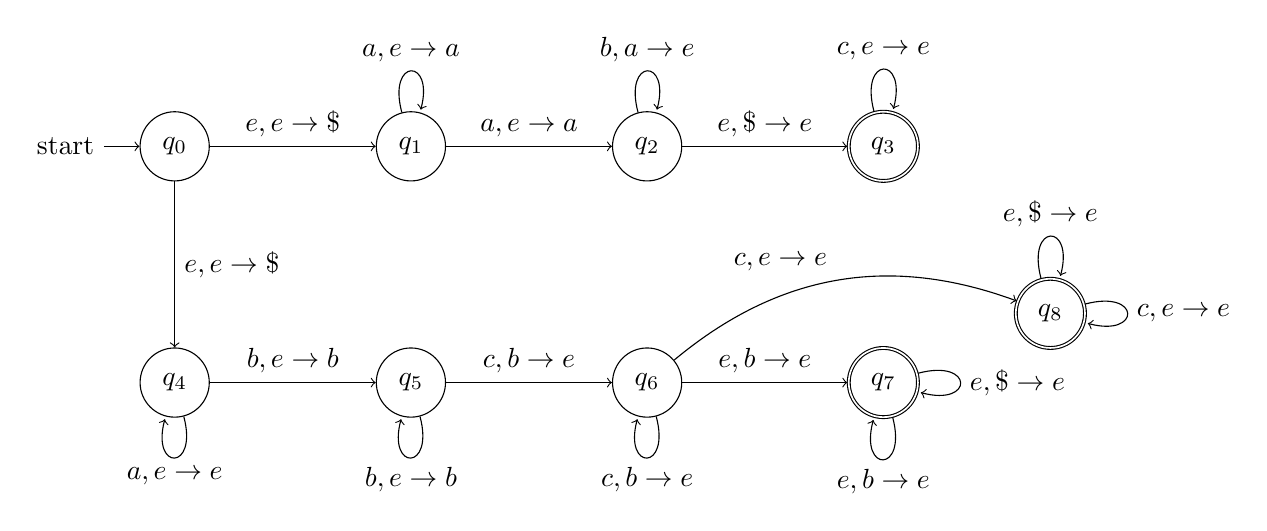
\begin{tikzpicture}[node distance=3cm,on grid,auto] 
				\node[state,initial   ]    (q0)                        {$q_0$};
				\node[state           ]    (q1) [right of=q0]          {$q_1$};
				\node[state           ]    (q2) [right of=q1]          {$q_2$};
				\node[state, accepting]    (q3) [right of=q2]          {$q_3$};
				\node[state           ]    (q4) [below of=q0]          {$q_4$};
				\node[state           ]    (q5) [right of=q4]          {$q_5$};
				\node[state           ]    (q6) [right of=q5]          {$q_6$};
				\node[state, accepting]    (q7) [right of=q6]          {$q_7$};
				\node[state, accepting]    (q8) [below right of=q3]    {$q_8$};
		
				\path [->]
				(q0) edge                node {$e,e \rightarrow \$$} (q1)
						 edge                node {$e,e \rightarrow \$$} (q4)
				(q1) edge                node {$a,e \rightarrow a$}  (q2)
						 edge [loop above]   node {$a,e \rightarrow a$}  ()
				(q2) edge                node {$e,\$ \rightarrow e$} (q3)
						 edge [loop above]   node {$b,a \rightarrow e$}  ()
				(q3) edge [loop above]   node {$c,e \rightarrow e$}  ()
				(q4) edge                node {$b,e \rightarrow b$}  (q5)
						 edge [loop below]   node {$a,e \rightarrow e$}  ()
				(q5) edge                node {$c,b \rightarrow e$}  (q6)
						 edge [loop below]   node {$b,e \rightarrow b$}  ()
				(q6) edge                node {$e,b \rightarrow e$}  (q7)
						 edge	[bend left=30] node {$c,e \rightarrow e$}  (q8)
						 edge [loop below]   node {$c,b \rightarrow e$}  ()
				(q7) edge [loop below]   node {$e,b \rightarrow e$}  ()
						 edge [loop right]   node {$e,\$ \rightarrow e$} ()
				(q8) edge [loop right]   node {$c,e \rightarrow e$}  ()
						 edge [loop above]   node {$e,\$ \rightarrow e$} ();
		
			\end{tikzpicture}
		\end{tabular}
		\item 
		% Sample empty table for your convenience, edit/use as you wish.
		
		\vspace{3cm}
		\begin{tabular}{|llrl|}
			\hline
			State & Input           & Stack & Transition             \\
			\hline
			$q_0$ & aabcc           & e     & -                      \\
			$q_4$ & aabcc           & \$    & {$e,e \rightarrow \$$} \\
			$q_4$ &  abcc           & \$    & {$a,e \rightarrow e$}  \\
			$q_4$ &   bcc           & \$    & {$a,e \rightarrow e$}  \\
			$q_5$ &    cc           & b\$   & {$b,e \rightarrow b$}  \\
			$q_6$ &     c           & \$    & {$c,b \rightarrow e$}  \\
			$q_8$ &     e           & \$    & {$c,e \rightarrow e$}  \\
			$q_8$ &     e           & e     & {$e,\$ \rightarrow e$} \\
						&                 &       & Accepts                \\
			\hline
		\end{tabular}
		% Sample empty table for your convenience, edit/use as you wish.
		% You are expected to trace all the possible computations
		\begin{tabular}{|llrl|}
			\hline
			State & Input           & Stack & Transition             \\
			\hline
			$q_0$ & bac             & e     & -                      \\
			$q_4$ & bac             & \$    & {$e,e \rightarrow \$$} \\
			$q_5$ &  ac             & b\$   & {$b,e \rightarrow b$}  \\
						&                 &       & Rejects                \\
			\hline
						&                 &       &                        \\
			\hline
			State & Input           & Stack & Transition             \\
			\hline
			$q_0$ & bac             & e     & -                      \\
			$q_1$ & bac             & \$    & {$e,e \rightarrow \$$} \\
						&                 &       & Rejects                \\
			\hline
		\end{tabular}
	\end{enumerate}

\section*{Answer 4}

\subsection*{a.}
	Let $M$ be the PDA equivalent to the CFG $G$ where $M = \Big(\{p,q\}, \Sigma, V, \Delta, p, \{q\}\Big)$ with
		\begin{align*}
			\Delta = & \{((p,e,e),(q,E)), & & (T1)  \\
							 & ((q,e,E),(q,E+T)), & & (T2)  \\
							 & ((q,e,E),(q,T)),   & & (T3)  \\
							 & ((q,e,T),(q,TxF)), & & (T4)  \\
							 & ((q,e,T),(q,F)),   & & (T5)  \\
							 & ((q,e,F),(q,(E))), & & (T6)  \\
							 & ((q,e,F),(q,a)),   & & (T7)  \\
							 & ((q,a,a),(q,e)),   & & (T8)  \\
							 & ((q,+,+),(q,e)),   & & (T9)  \\
							 & ((q,x,x),(q,e)),   & & (T10) \\
							 & ((q,(,(),(q,e)),   & & (T11) \\
							 & ((q,),)),(q,e))\}  & & (T12).
		\end{align*}

\subsection*{b.}
		\qquad We know by Lemma 3.4.2 that we can convert a PDA $M$ to $M''$ such that $M = M''$ and $M''$ is \textbf{simple}. So by not executing the last step of this lemma, we can acquire a PDA $M''$ which has $|\beta| \leq 1 \text{ and } |\gamma| \leq 1$. After this, we can consider each $\Delta''$ transition that in form $((q,x,\beta), (p, \gamma))$ where $|\beta|,|\gamma| \neq 0$ and replace it with $((q,x,\beta), (r, e)) \text{ and } ((r,e,e), (p, \gamma))$ where $x \in \Sigma$. Thus create $\Delta'$ and $K'$ for PDA $M'$ which has $|\beta|+|\gamma| \leq 1$.


\section*{Answer 5}

\subsection*{a.}
\begin{enumerate}[(i)]
\item 
	\qquad Consider context-free grammar
		$$\ G = \Big(V=\{S_1\}, \Sigma=\{a, b\}, R = \{S_1 \rightarrow aS_1b\ |\ e\}, S_1\Big) \text{ where } L(G) = \{a^nb^n : n\geq0\}$$
	\qquad Notice that $a^mb^{m+n}a^n$ is concatenation of $a^mb^m$ and $b^na^n$ and both of these can be generated by $G$. Since context-free languages are closed under concatenation, $a^mb^{m+n}a^n$ is context-free.
\item 
	%\vspace*{-1.5cm}
	Let
	\begin{minipage}{0.4\textwidth}
		%\vspace*{2.1cm}
		$$S_1 \rightarrow bS_2\ |\ bS_3aa$$
		$$S_2 \rightarrow AS_2a\ |\ b$$
		$$S_3 \rightarrow aS_2A\ |\ b$$
		$$S_4 \rightarrow aA\ |\ a$$
	\end{minipage}
	in 
	\begin{minipage}{0.5\textwidth}
		$\ G = \Big(V=\{S_1, S_2, S_3, A\}, \Sigma=\{a, b\}, R, S_1\Big)$.
	\end{minipage}\\

	$\{a,b\}^*-L = \overline{L} = a\Sigma^* \cup \Sigma^*a \cup \Sigma^*bb\Sigma^* \cup G$ and since we know all these languages are context-free, $\{a,b\}^*-L$ is context-free.
\end{enumerate}

\subsection*{b.}
\begin{enumerate}[(i)]
\item 
	\qquad Assume given language be context-free. Then there exists a split $uvxyz$ such that it is in the language. Let $p$ be the pumping length and consider string $a^{p^2}b^p$.
	\begin{center}
		Case 1, there are only $a$'s in $v$ and $y$: The string $uv^2xy^2z$ has the property $p^2+2k \leq p^2$ where $vxy \leq p$ and $2k > 0$ so it can not be in the language.\\
		Case 2, there are only $b$'s in $v$ and $y$: The string $uv^0xy^0z$ has the property $p^2 \leq p^2-2k$ where $vxy \leq p$ and $2k > 0$ so it can not be in the language.\\
		Case 3, there are both $a$'s and $b$'s in $vxy$: The string has the property $p^2 - k \leq (p-j)^2$ where $vxy \leq p$ and $j+k > 0$ with $k$ is the number of $a$'s $j$ is the number of $b$'s.
	\end{center}
	\vspace{-0.4cm}
	$$j+k \leq p,\ j \leq p-k,\ j>0,\ k>0$$
	$$p^2 - k \leq p^2 - 2pj +j^2,\ p^2 - k \leq p^2 - 2p(p-k) + (p-k)^2$$
	$$p^2 - k \leq k^2 \text{ is false because } j^2 + 2jk + k^2 \leq p^2$$
	Since every case considered builds up to a contradiction, this language is not context-free.

\item 
	\qquad Let $L$ be the given language and $L' = L \cap a^*ba^*ba^*b = \{a^nba^nba^n \in \{a,b\}^*\ |\ n\geq 0\}$. Not that if $L$ is context-free, then $L'$ must be too by closure properties. Assume $L'$ is context free. Then there exists a split $uvxyz$ such that it is in $L'$. Let $p$ be the pumping length and consider string $a^pba^pba^pb$.
	\begin{center}
		Case 1, there is a $b$ in $vxy$: The string $uv^2xy^2z$ has more than three $b$'s so it can not be in the language.\\
		Case 2, there are only $a$'s in $v$ and $y$: The string $uv^2xy^2z$ has \textbf{at least} one group of $a$'s not matching other(s) so it can not be in the language. This case is also valid when $v$ and $y$ consists different $a$ groups divided with a $b$ i.e. $x = b$. "at least" is emphasised for that purpose.
	\end{center}
	\qquad Since we found that $L'$ is not a context-free language, we can conclude $L$ is not also.
\end{enumerate}


\section*{Answer 6}
% You do not need to explain the following
\begin{enumerate}[(i)]
\item (T/F)? False.
\item (T/F)? True.
\item (T/F)? True.
\item (T/F)? False.
\end{enumerate}

% Please do not submit your answers to the ungraded questions.
% Hope you have fun :) 
\end{document}

​

